\documentclass[12pt]{article}
\usepackage{a4wide, amsfonts, epsfig}
\newcommand\soln{\noindent\textit{Solution:} }


%skyline stuff
\font\upright=cmu10 scaled\magstep1
\setlength{\unitlength}{0.012500in}
\begingroup\makeatletter\ifx\SetFigFont\undefined
\def\x#1#2#3#4#5#6#7\relax{\def\x{#1#2#3#4#5#6}}%
\expandafter\x\fmtname xxxxxx\relax \def\y{splain}%
\ifx\x\y   % LaTeX or SliTeX?
\gdef\SetFigFont#1#2#3{%
  \ifnum #1<17\tiny\else \ifnum #1<20\small\else
  \ifnum #1<24\normalsize\else \ifnum #1<29\large\else
  \ifnum #1<34\Large\else \ifnum #1<41\LARGE\else
     \huge\fi\fi\fi\fi\fi\fi
  \csname #3\endcsname}%
\else
\gdef\SetFigFont#1#2#3{\begingroup
  \count@#1\relax \ifnum 25<\count@\count@25\fi
  \def\x{\endgroup\@setsize\SetFigFont{#2pt}}%
  \expandafter\x
    \csname \romannumeral\the\count@ pt\expandafter\endcsname
    \csname @\romannumeral\the\count@ pt\endcsname
  \csname #3\endcsname}%
\fi
\fi\endgroup

\begin{document}
\begin{center}
{\bf 2E2 Tutorial Sheet 13 Second Term}\footnote{Conor
Houghton, {\tt houghton@maths.tcd.ie} and {\tt
http://www.maths.tcd.ie/\char126 houghton/ 2E2.html}}
\\[1cm]
5 Febuary 2006
\end{center}
{
\begin{enumerate}
\item (2) An equation system has solution
\begin{equation}
\left(\begin{array}{c}y_1\\y_2\end{array}\right)=c_1\left(\begin{array}{c}1\\2i\end{array}\right)e^{2it}+c_2\left(\begin{array}{c}1\\-2i\end{array}\right)e^{-2it}
\end{equation}
Sketch the phase diagram.
\vskip .5cm \soln So our statedgy with complex solutions is to examine
trajectories starting at $y_1(0)=r$ and $y_2(0)=0$, since the complex
solutions always give ellipses, circles or spirals, looking at these
trajectories is enough to sketch the whole phase diagram. In this case
we expect a circle node with elliptical trajectories. Putting in the initial conditions we get
\begin{equation}
\left(\begin{array}{c}r\\0\end{array}\right)=c_1\left(\begin{array}{c}1\\2i\end{array}\right)+c_2\left(\begin{array}{c}1\\-2i\end{array}\right)
\end{equation}
so
\begin{eqnarray}
c_1+c_2&=&r\cr
2ic_1-2ic_2&=&0
\end{eqnarray}
giving $c_1=c_2=r/2$. Now, substitute this back in 
\begin{equation}
\left(\begin{array}{c}y_1\\y_2\end{array}\right)=\frac{r}{2}\left(\begin{array}{c}1\\2i\end{array}\right)e^{2it}+\frac{r}{2}\left(\begin{array}{c}1\\-2i\end{array}\right)e^{-2it}
\end{equation}
and using 
\begin{eqnarray}
e^{2it}&=&\cos{2t}+i\sin{2t}\cr
e^{-2it}&=&\cos{2t}-i\sin{2t}
\end{eqnarray}
this gives the real expression
\begin{equation}
\left(\begin{array}{c}y_1\\y_2\end{array}\right)=\left(\begin{array}{c}r\cos{2t}\\-2r\sin{2t}\end{array}\right)
\end{equation}
\vskip .5cm
This is an ellipse, it is easy to see that it satisfies the ellipse equation
\begin{equation}
y_1^2+\left(\frac{y_2}{2}\right)^2=r^2
\end{equation}
The factor of two on the $y_2$ means it goes twice as far in this direction. For very small $t$ $y_2$ is negative so the trajectory starts off downwards. Hence we have a circle node with elliptical clockwise trajectories.
\begin{center}
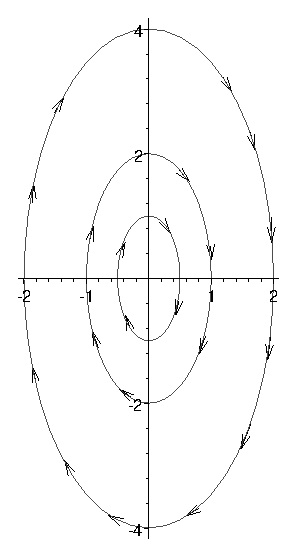
\epsfig{file=ellipse2.eps,width=5cm}
\end{center}
\vskip 1cm
\item (3) Find the general solution for the system
\begin{eqnarray}
\frac{dy_1}{dt}&=&3y_1+y_2\\
\frac{dy_2}{dt}&=&-y_1+y_2
\end{eqnarray}
\vskip .5cm
\soln This is one of those systems where there is only one eigenvalue and only one eigenvector, $\lambda=2$ with 
\begin{equation}
{\bf x}=\left(\begin{array}{c}1\\-1\end{array}\right)
\end{equation}
so the solution is of the form
\begin{equation}
{\bf y}=c_1{\bf x}e^{2t}+c_2\left(t{\bf x}+{\bf u}\right)e^{2t}
\end{equation}
where you need to find ${\bf u}$ by substituting 
\begin{equation}
{\bf y}=\left(t{\bf x}+{\bf u}\right)e^{2t}
\end{equation} 
back into the equation.  This means the ${\bf u}$ vector in
the extra solution is the solution to 
$$
\left(\begin{array}{cc}1&1\\-1&-1\end{array}\right){\bf u}=
\left(\begin{array}{c}1\\-1\end{array}\right).
$$
Writing 
$${\bf u}=\left(\begin{array}{c}a\\b\end{array}\right)
$$
gives equations
\begin{eqnarray*}
a+b&=&1\\
-a-b&=&-1
\end{eqnarray*}
These two equations are the same, as you expect, and if $b=0$ then $a=1$. Thus, \vskip .5cm
the general solution is
$$
{\bf y}=c_1\left(\begin{array}{c}1\\-1\end{array}\right)e^{2t}+c_2\left[\left(\begin{array}{c}1\\-1\end{array}\right)t+\left(\begin{array}{c}1\\0\end{array}\right)\right]e^{2t}
$$
or
$${\bf y}=\left[(c_1+c_2t)\left(\begin{array}{c}1\\-1\end{array}\right)+c_2\left
(\begin{array}{c}1\\0\end{array}\right)\right]e^{2t}.
$$
\vskip 1cm
\item (3) Find the solution for the system
\begin{eqnarray*}
y_1'&=&4y_1+y_2\\
y_2'&=&-y_1+2y_2.
\end{eqnarray*}
with initial conditions $y_1(0)=3$ and $y_2(0)=2$.
\vskip .5cm
\soln \begin{equation}
A=\left(\begin{array}{cc}4&1\\-1&2\end{array}\right)
\end{equation}
and there is only one eigenvector,
\begin{equation}
{\bf x}=\left(\begin{array}{c}-1\\ 1\end{array}\right)
\end{equation}
with eigenvalue $\lambda=3$. The solution is 
\begin{equation}
{\bf y}=c_1{\bf x}e^{\lambda t}+c_2(t{\bf x}+{\bf u})e^{\lambda t}
\end{equation}
where ${\bf u}$ satisfies
\begin{equation}
\left(A-\lambda{\bf 1}\right){\bf u}={\bf x}
\end{equation}
and so, in this case,
\begin{equation}
\left(\begin{array}{cc}1&1\\-1&-1\end{array}\right){\bf u}=\left(\begin{array}
{c}-1\\ 1\end{array}\right)
\end{equation}
and a solution to this is 
\begin{equation}
{\bf u}=\left(\begin{array}{c}-1\\ 0\end{array}\right)
\end{equation}
and so the solution is
\begin{equation}
{\bf y}=c_1\left(\begin{array}{c}-1\\ 1\end{array}\right)
e^{3 t}+c_2\left[
t\left(\begin{array}{c}-1\\ 1\end{array}\right)
+\left(\begin{array}{c}-1\\ 0\end{array}\right)
\right]e^{3 t}
\end{equation}
\vskip .5cm
Now, putting $t=0$ we get
\begin{equation}
\left(\begin{array}{c}3\\2\end{array}\right)=c_1\left(\begin{array}{c}-1\\ 1\end{array}\right)+c_2\left(\begin{array}{c}-1\\ 0\end{array}\right)
\end{equation}
and, hence,
\begin{eqnarray}
3&=&-c_1-c_2\cr
2&=&c_1
\end{eqnarray}
aso $c_2=1$ and $c_2=-5$ giving
\begin{equation}
{\bf y}=2\left(\begin{array}{c}-1\\ 1\end{array}\right)
e^{3 t}-5\left[
t\left(\begin{array}{c}-1\\ 1\end{array}\right)
+\left(\begin{array}{c}-1\\ 0\end{array}\right)
\right]e^{3 t}
\end{equation}
or
\begin{eqnarray}
y_1&=&(3+5t)e^{3t}\cr
y_2&=&(2-5t)e^{3t}
\end{eqnarray}
\end{enumerate}
}
\end{document}



